\chapter{ISPs as adversaries}\label{sec:attack_isp}

Of great importance to our approach, is aquiring real-time network traffic,
with downstream throughput being our only focus; here discuss the potential
scenarios that allow adversaries to obtain such information, and describe how,
in particular ISPs, could make use of it, to identify video streaming and
profile users based on their streaming habits.

\section{Attack Scenarios}\label{attack_scenarios}

Given the nature of modern Internet infrastructure, an adversary interested in
eavesdropping a particular communication, only needs to compromise a node on
the path the communication travels through. An \emph{on-path} attacker could
easily gain passive access to network and transport layers, and start capturing
network traffic. This can include malicious or compromised Wi-Fi access
points, routers, tapped network cables and ISPs. 

Rather than just attacking physical devices, leaks of information could occur
in network connections, in which an attacker physically close to the victim,
could make use of a \emph{Wi-Fi sniffer} to estimate traffic by capturing
physical layer WLAN packets.  Information may be encrypted by 802.11, and the
sniffer may not take into account packet retransmissions at the session layer
nor multiple TCP/IP flows on the same link, potentially causing noise on the
observation. Despite so, Reed et Al. \cite{leaky_streams}, have shown that it
is still possible to estimate WAP-to-client throughput and use it to identify
the content being streamed.

In addition to the above, \emph{side-channel eavesdropping} can exploit
information about the network structure, to saturate a link between the user
and the server, and estimate fluctuations of congestion by sending probes
remotely and observing queueing delays in routers \cite{side_channel}. 

We will now present the relevant phases and tools needed for an ISP to perform
such attack.

\section{Video Fingerprinting}

Assuming that the ISP has no direct access to the CDN titles are stored in, it
needs to build a database of video traffic to match against future video stream
captures. To build such a database, the ISP needs to have access to a network
interface, control its inbound bandwidth, (to get different levels of quality
for each title), and capture incoming traffic passing through it.

In order to control the incoming bandwidth, the ISP could either limit it
directly onto a generic L4 switch (probably more stable), or decide to connect
any UNIX-like machine and throttle the throughput of its main ethernet
interface. We will consider the scenario in which the ISP limits the bandwidth
of the ethernet interface of the switch.

The value of the enforced bandwidth determines the quality (bitrate) of the
content that will be captured. Assuming that each title has a unique bitrate
ladder, the ISP should come up with an ad-hoc policy for every video to
faithfully reconstruct the quality levels of it. While correct, a more viable
approach to this problem, would be to just consider a range of bitrates capable
of spanning the space of possible quality levels. 

In our own version of the attack, presented in \Cref{sec:approach}, we use
the values in \Cref{tab:bandwidths}. 

\begin{table}[htb]
  \centering
  \begin{tabular}{|c|c|c|c|c|c|c|c|c|c|c|c|c|}
    \hline
    \multicolumn{13}{|c|}{\textbf{Bandwidth levels (Mbps)}} \\
    \hline
    0.6 & 0.8 & 1.2 & 2 & 3.5 & 4.2 & 4.8 & 5.5 & 6.5 & 7.05 & 10 & 15 & 20 \\ 
    \hline
  \end{tabular}
  \caption{Enforced bandwidth levels.}
  \label{tab:bandwidths}
\end{table}

The ISP can now connect a UNIX-like machine to the switch's network interface
with bandwidth limit \emph{b}, and invoke \texttt{adudump} to infer the size of
each \emph{application data unit} ADU by processesing TCP/IP packet header
traces that generate \emph{a-b-t connection vectors} \cite{hernandez}.

\subsection{The a-b-t model}

\todo{Describe the model}

\subsection{Inference}

\todo{Describe how ADUs size are computed}

\begin{figure}[!htb]
  \centering
  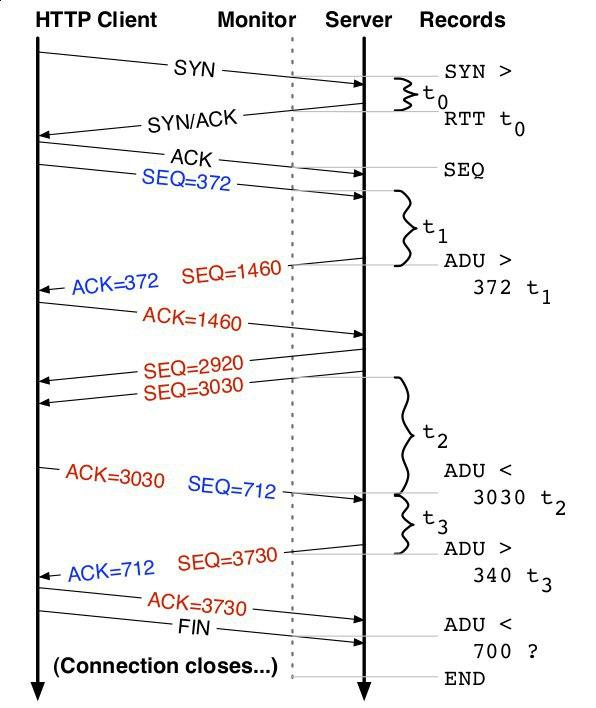
\includegraphics[width=0.7\columnwidth]{img/adudump.png}
  \caption{Detailed segment size inference in adudump.}
  \label{fig:adudump}
\end{figure}

\todo{Add sample adudump trace}

In addition, to identify specific video traffic from a Netflix CDN, the ISP
could either inspect the DNS response packets or TLS handshake messages, and
perform a DNS lookup for each video every time, or to maintain an updated list
of IP addresses with mappings to the recorded traffic.

\section{Capturing video traffic}

This, requires the ISP to be in possess of a generic L4 switch that can mirror
traffic from a port to another one. Then any UNIX-like system that implements
\emph{libpcap} is suitable for capturing inbound traffic on the mirrored port, as
presented below in \Cref{fig:schema}.

\begin{figure}[!htb]
  \centering
  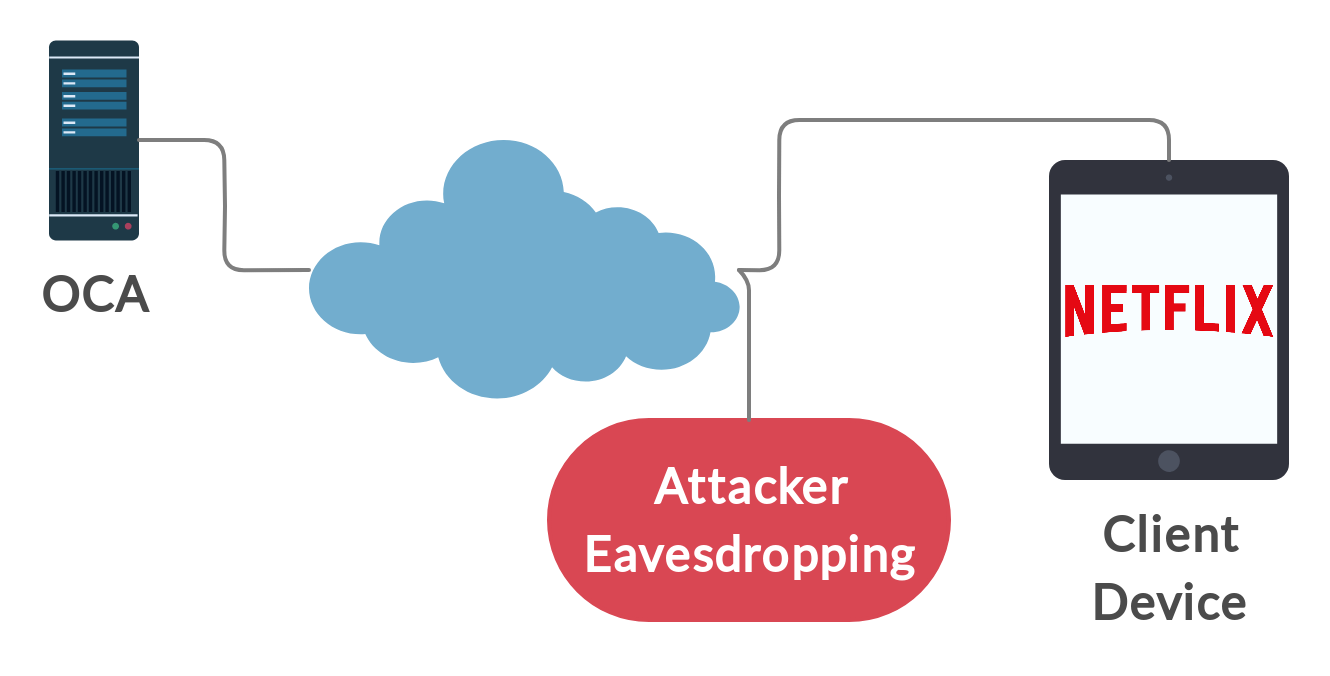
\includegraphics[width=0.9\columnwidth]{img/schema.png}
  \caption{Traffic capture scenario.}
  \label{fig:schema}
\end{figure}

